\subsubsection{Drools}

Kobold bietet seinem Benutzer einen Workflow-Mechanismus, der die Wahrung des definierten produktlinien-basierten 
Entwicklungsprozesses unterst�tzt. Dieser f�hrt Konsistenzpr�fungen durch, die in anderen Client-Instanzen 
automatisch Workflows  ansto�en, um die Inkonsistenz zu beheben.
Zur Realisierung des Workflow-Mechanismus wird die Rule Engine Drools\footnote{http://www.drools.org} 
verwendet.\par
Daf�r wird eine Regelbasis in XML f�r Drools erzeugt. Diese besteht aus einer Menge aller Regelmengen und 
befindet sich auf dem Server. Eine Regelmenge wiederum besteht aus Regeln. Eine solche Regel gliedert 
sich in drei Teile: Parameter, Bedingung und Konsequenz. Dabei bilden die Parameter eventuell ben�tigte 
Parameter f�r die Regel. Die Bedingung �berpr�ft, ob die Regel angewendet wird oder nicht. Die Konsequenz
beeinhaltet die Aktionen, die durchgef�hrt werden, falls die Bedingung erf�llt ist.\par

Der Workflow-Mechanismus spielt sich sowohl auf dem Kobold Server als auch auf dem Kobold Client ab.\par

\paragraph{Aktionen auf dem Kobold Server}
F�hrt ein Client eine Aktion aus, so wird diese dem Kobold Server gemeldet. Dieser wendet die Aktion als Fakt
auf die Regelbasis an, die sich auf dem Server befindet. Ein Fakt ist dabei eine Mitteilung an den Server. 
Es werden dabei alle Regeln durchlaufen. Stimmt das 
Ereignis mit der Bedingung einer Regel �berein, so 
wird die Konsequenz dieser ausgef�hrt. Die Ergebnisse dieser Regelkonsequenzen werden zu einem 
Workflow-Objekt zusammengef�gt (zum Beispiel eine Reihe von Anweisungen). Ein Workflow-Objekt ist dabei 
eine Art XML-Struktur, die einen Titel und eine Liste aller Regelresultate 
besitzt. Diese Workflow-Objekt wird 
dann auf die Message-Queues der Clients gelegt, f�r die das Workflow-Objekt relevant ist. 

\paragraph{Aktionen auf dem Kobold Client}
Sobald der Client eine Aktion ausf�hrt, meldet er diese dem Kobold Server um m�gliche Inkonsistenzen zu 
vermeiden. Wird ein Workflow entwickelt, so bekommt jeder Kobold Client, der den Workflow ansto�en sollte,
beim n�chsten Login dieses Objekt gepollt. Der Anwender wird dar�ber in der Workflow-View des Kobold Clients
informiert.\newline
\newline
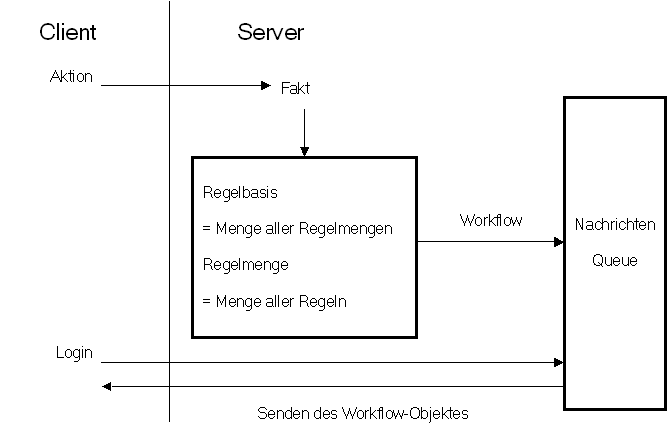
\includegraphics[width=15cm]{drools.png}\newline

\paragraph{Die Regelbasis in Kobold}
Kobold wird in dieser Iteration eine Anfangsregelbasis zur Verf�gung stellen, die vom Anwender jederzeit erweitert werden 
kann. Er muss dabei eine neue Regel erstellen und sie der Regelbasis hinzuf�gen. Diese Regeln m�ssen dann 
nicht unbedingt zum 
Workflow-Objekt hinzugef�gt werden, sondern k�nnen in ihrer Konsequenz auch andere Aktionen ausf�hren. 
Dies bleibt dem Anwender �berlassen. Zur Erstellung einer neuen Regel wird ihm au�erdem ein Editor 
zur Verf�gung stehen, 
der in einer der kommenden Iterationen entstehen wird. 